\documentclass[tikz]{standalone}

\usetikzlibrary{arrows.meta,positioning}

\begin{document}
	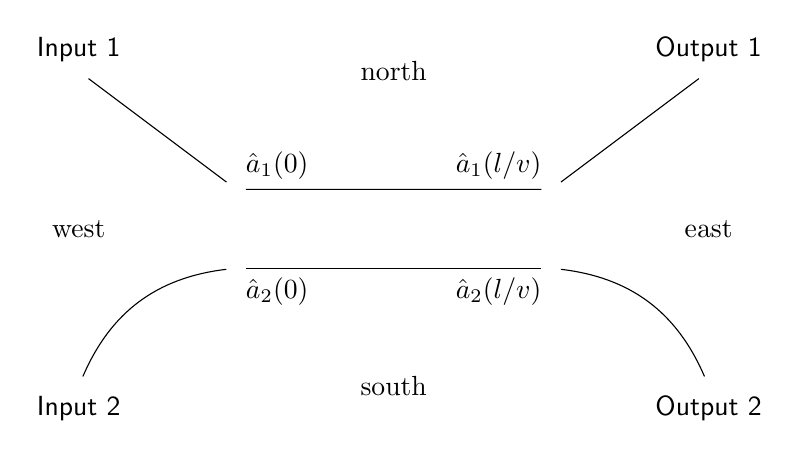
\begin{tikzpicture}[
		node distance=4em,
		arrow/.style={-latex},
		block/.style={draw, very thick, fill=white, minimum height=12ex, minimum width=6em, align=center},
	]
		\draw (0,0) node(in1){} node[above]{\textsf{Input 1}};
		\draw (8,-4) node(out2){} node[below]{\textsf{Output 2}};
		\draw (in1-|out2) node(out1){} node[above]{\textsf{Output 1}};
		\draw (in1|-out2) node(in2){} node[below]{\textsf{Input 2}};
		
		\path (in1) -- (in2) node[midway] (west) {west};
		\path (in1) -- (out1) node[midway] (north) {north};
		\path (out1) -- (out2) node[midway] (east) {east};
		\path (in2) -- (out2) node[midway] (south) {south};
		
		\draw (west) ++(2,0.5) node(A){} node[above right]{$\hat{a}_1(0)$};
		\draw (east) ++(-2,-0.5) node(C){} node[below left]{$\hat{a}_2(l/v)$};
		\draw (A|-C) node(D){} node[below right]{$\hat{a}_2(0)$};
		\draw (A-|C) node(B){} node[above left]{$\hat{a}_1(l/v)$};
		
		\draw (in1) -- (A) -- (B) -- (out1);
		\draw (in2) edge[bend left] (D)
		        (D) edge (C)
		        (C) edge[bend left] (out2);
	\end{tikzpicture}
\end{document}
